\ctable[
  cap = Impedance Element Summary,
  caption = A Summary of Elements Which Provide an Impedance,
  label = tab:impedanceSummary,
  pos = h
]{lVVV}{
  \tnote{Typical ceramic capacitors. Electrolytic capacitors have larger capacitance.}
  }{
  \FL
  & Capacitor                     & Inductor                & Resistor                     \\
  \midrule \vspace{-1em}\\ \vspace{-0.25em}
  Symbol
  & 
\includegraphics[height=30pt]{figures/capacitor} 
  & 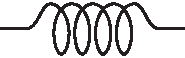
\includegraphics[height=30pt]{figures/inductor} 
  & 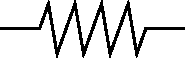
\includegraphics[height=30pt]{figures/resistor} \\
  Unit & Farad (F) & Henry (H) & Ohm ($\Omega$)      \\ \vspace{0.25 em}
  Typical Values
  & 0.1 pF -- 0.5 mF\tmark
  & 0.1 $\mu$H -- 10 mH
  & 10 $\Omega$ -- 1 G$\Omega$ \\ \vspace{0.5 em}
  Impedance
  & $\displaystyle Z_C=\frac{1}{j \omega C}$
  & $\displaystyle Z_L = j \omega L$
  & $\displaystyle Z_R = R$                    \\ 
  Energy Storage
  &  $\displaystyle E_C = \frac{1}{2} CV^2$
  & $\displaystyle E_L = \frac{1}{2}Li^2$
  & N/A 
\LL
}

